% ==================================================
% CHAPTER 6: Using x-rays to measure relative strip position offsets
% ==================================================

\chapter{Using x-rays to measure relative strip position offsets}
\label{chap:xray}

Local offset measurements were done with the x-ray method. The reader is referred to the paper describing the x-ray method~\cite{lefebvre_precision_2020}, although some minor changes have been made to the experimental setup since it was written. The experimental setup described here is current and was used to collect the data presented in this thesis.
% Makesure to put this in the statement of contribution

% NOTE: Wrote this with information available in JINST, or things I know to be updated (eg. brass holder and collimator). I can guess at other things based on the WedgeAlignment-Production code, but don't actually know. Those things are in iffalse statements.
% --------------------------------------------------
\section{Experimental setup}
% --------------------------------------------------

The x-ray tests were performed after the quadruplets arrived at CERN, were assembled into wedges, and alignment platforms installed. Essentially, an x-ray gun was attached to one of the alignment platforms glued to the surface of the wedge and the x-ray beam profile recorded by the strips.

\begin{figure}
    \centering
    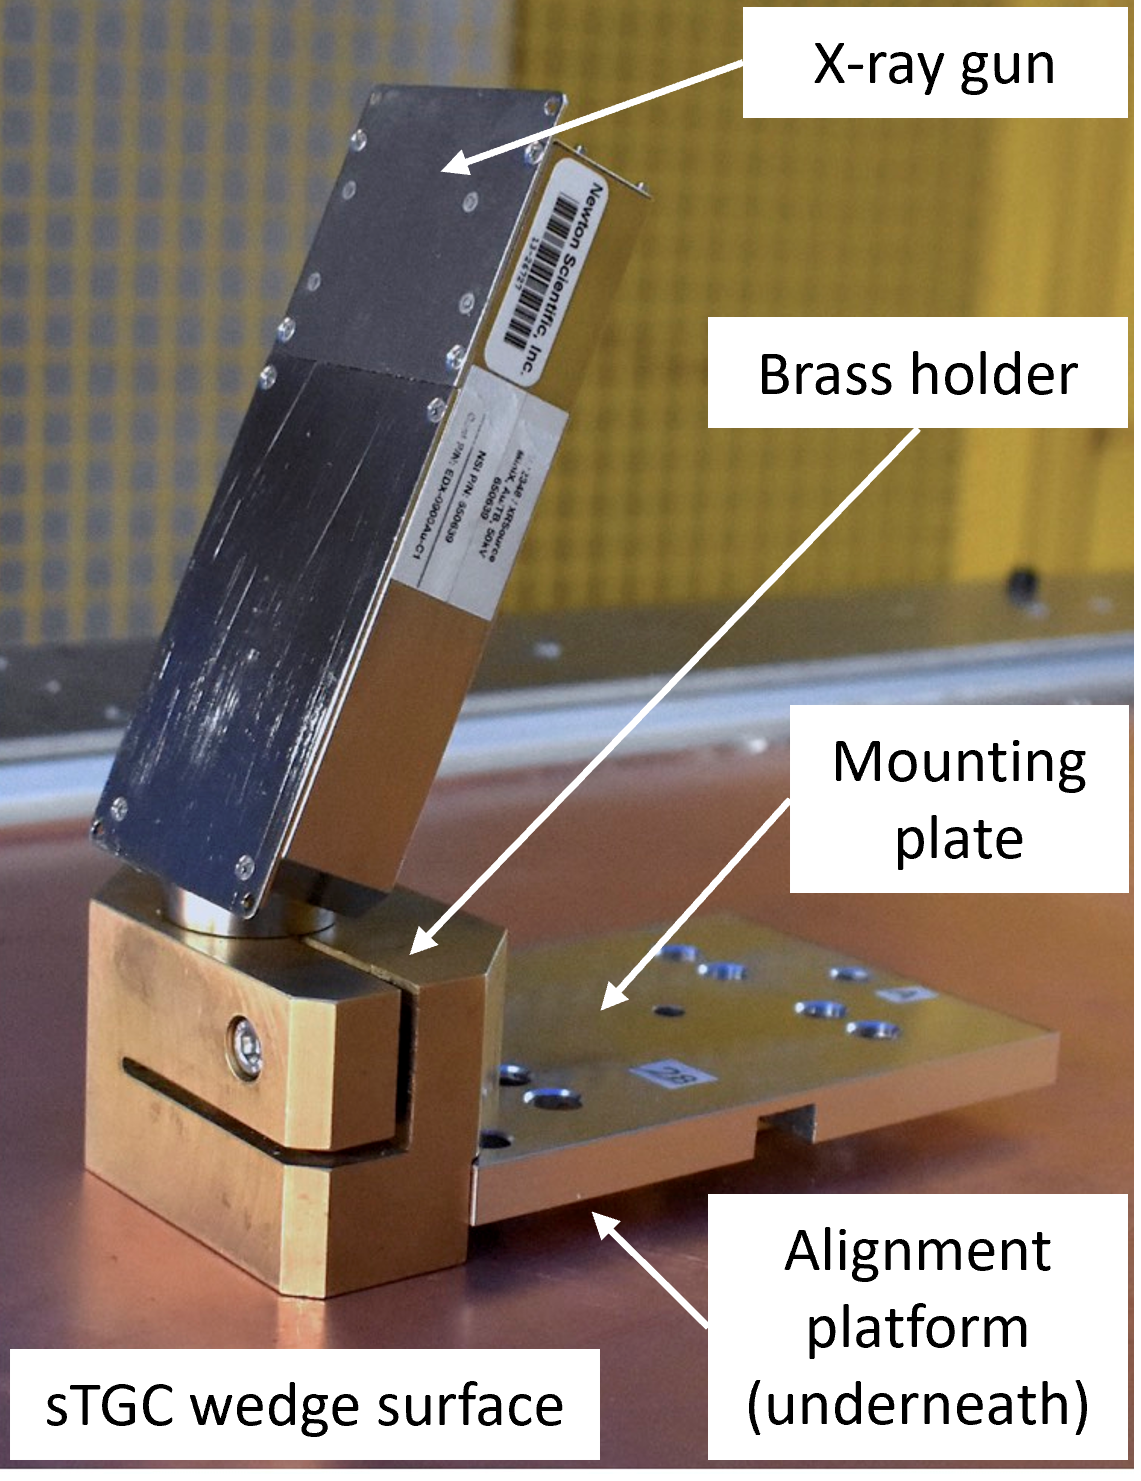
\includegraphics[width = 0.5\textwidth]{figures/xray_setup.png}
    \caption{The x-ray gun mounted to the alignment platform on the surface of the wedge. Adapted from~\cite{lefebvre_precision_2020}.}
    \label{fig:xray_setup}
\end{figure}

The wedges were installed on carts that could rotate their surface to a horizontal position. A mounting platform was installed on top of the alignment platform using a three-ball mount. The x-ray gun used was an \href{https://www.amptek.com/-/media/ametekamptek/documents/resources/specs/mini-x-specifications.pdf?la=en\&revision=512f7eb3-01b3-47fd-864f-5525c850fc6e\&hash=B8B03C0592486E2D91C566C4326F15F5}{Amptek Mini-X tube}. The gun was placed in a brass holder with built-in \SI{2}{mm} collimator and \SI{280}{\micro\meter} copper filter. The holder was mounted on one of five positions on the mounting platform, as shown in figure~\ref{fig:xray_setup}. Gun positions were chosen to avoid wire support structures in the sTGCs that reduce hit efficiency~\cite{lefebvre_thesis} and boundaries between sets of strips read out by two different ASICs that could each have different thresholds. 

As with cosmics data collection, each sTGC also needed gas and high voltage to operate. Each layer was operated at \SI{2.925}{kV} with high voltage from a NIM crate. The chambers were flushed with CO$_2$ before and during data collection.

% The copper filter helped to reduce the effect of attenuation non-uniformities.
The gun produced x-rays with energies under \SI{40}{\kilo\electronvolt} with peaks in the 7-\SI{15}{keV} range. \iffalse Peaks in the 0-\SI{30}{keV} range were filtered out by the copper filter and the copper of the sTGCs. \fi The x-rays mostly interacted with the wedge's copper electrodes and gold-plated tungsten wires via the photo effect. The resulting photoelectrons caused ionization avalanches that were picked up by the strips.
% During ATLAS operation, the position of the source plates will be monitored using the new alignment system~\cite{nsw_tdr}. Therefore, their position will be known in the absolute ATLAS coordinate system. 

% --------------------------------------------------
\section{Data acquisition}
% --------------------------------------------------

A different version of the same front end electronics, but the same ASIC, as used in cosmics testing were used for the x-ray testing to amplify the data and measure the peak signal amplitude. Data was collected for two minutes per gun position with random triggers. A trigger recorded all signals above threshold. \iffalse within \SI{75}{ns} and the signals on neighbouring strips.\fi  Pad and wire data was not recorded.
% Neighbour triggering based on my understanding of the analysis. Does not actually matter for these purposes.

% --------------------------------------------------
\section{Data preparation}
% --------------------------------------------------

Like with cosmics analysis, a default pedestal is subtracted from the signal peak amplitude on each electrode.

Clusters are defined as groups of contiguous strip hits collected within \SI{75}{ns}. The peak signal amplitude of each electrode in a cluster is fit with a Gaussian, and the mean of the Gaussian is taken as the cluster position. Cluster positions are corrected for DNL (see definition in appendix~\ref{appendix:systematics_dnl}). Only clusters composed of hits on 3-5 strips were used in the x-ray analysis. Clusters with signal on more than 5 strips were cut because they were most likely caused by photoelectrons ejected with enough energy to  \iffalse cause more primary ionization and subsequent avalanches ( \fi be $\delta$-rays.
% Note: analysis definitely does the double cluster cut

The x-ray analysis diverges entirely from the cosmics analysis algorithm here because the x-rays do not leave tracks. The signals picked up by the strips are from photoelectrons liberated from the metals of the sTGCs, which only travel through one gas volume and are ejected at all angles. Instead of creating tracks, the cluster position distribution on each layer is used to define the beam profile. A typical beam profile is shown in figure~\ref{fig:xray_beam_profile}.

\begin{figure}
    \centering
    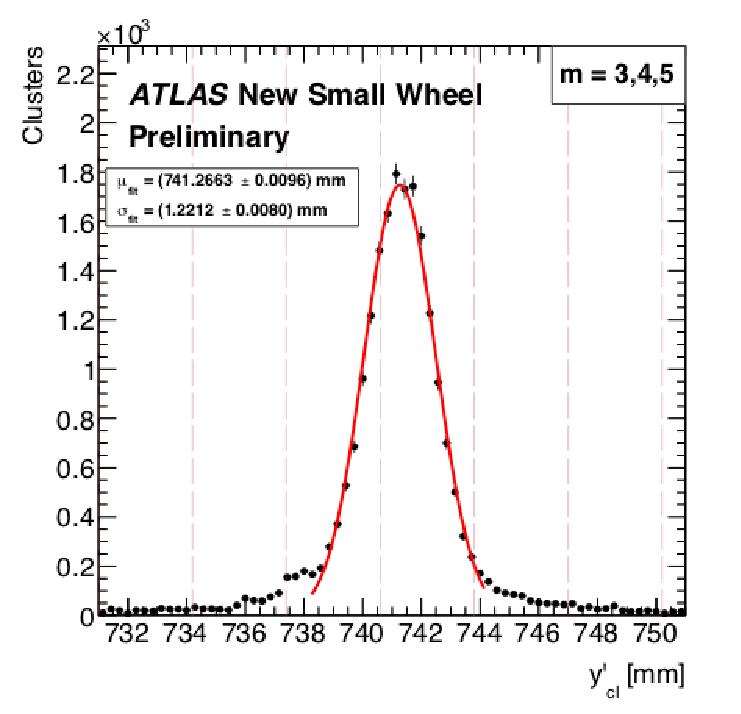
\includegraphics[width = 0.5\textwidth]{figures/figure_xray_beam_profile.pdf}
    \caption{Distribution of x-ray cluster mean positions after the analysis cuts and corrections. The strip cluster multiplicity, $m$, was limited to 3, 4 and 5. The red curve is a Gaussian fit of the distribution and the pink dashed lines denote the edges of the strips~\cite{lefebvre_precision_2020}.}
    \label{fig:xray_beam_profile}
\end{figure}

% --------------------------------------------------
\section{Measuring local offsets}
% --------------------------------------------------
The mean of the cluster position distribution is taken as the x-ray beam profile center. The expected center is calculated assuming a wedge with nominal geometry given the gun position, corrected for: the geometry of the brass holder, the positioning and angle of the alignment platforms and the beam angle. The difference between the expected and reconstructed beam profile center is a measure of the local offset. Applying the logic of equation~\ref{eqn:local_translation} to the beam profile, the Gaussian mean of cluster positions on the given layer acts as the recorded position, $y_i$, the expected center is $y_{nom, i}$ and the local offset is $d_{local, i}$ as before, where $i$ denotes the layer. Since the position of the alignment platforms will be monitored by the alignment system in ATLAS~\cite{nsw_tdr}, the position of the strips that should have been at he gun position are shifted by $d_{local, i}$ and so are known in the ATLAS coordinate system for every position where x-ray data was taken.

The x-ray working group accepted an uncertainty of \SI{120}{\micro\meter} on the beam profile centers. The largest uncertainty comes from the effect of the gun angle, which proved difficult to measure and correct for.

The local offsets are not presented here as the author did not conduct this work. However, the author used the local offsets to calculate relative local offsets.

% --------------------------------------------------
\section{Measuring relative local offsets}
% --------------------------------------------------

The x-ray local offsets were shown to be correlated with the local offsets calculated from the CMM data, but the CMM data does not include the effect of inter-layer misalignments so the degree of correlation measurable was limited. Cosmics data is affected by inter-layer misalignments. Since the local offsets for x-rays and cosmics data are measured in different coordinate systems, they cannot be compared directly. Bringing the cosmics relative local offsets into an absolute coordinate system is impossible; however, the x-ray local offsets can be brought into a relative coordinate system.

The measured x-ray beam profile centers were systematically affected by local offsets in the same way as the mean cosmics residuals, as modeled by equation \ref{eqn:local_translation}. Therefore, if a 2-layer track is built from the beam profile centers on each layer and the residual calculated on a third layer, that residual should match the local mean cosmics residual. The residual is the difference between the beam profile center on the layer of interest and the polated track position from the beam profile centers recorded on the two fixed layers. The beam profile center on the layer of interest acts as $y_{i}$ and the polated track position acts as $y_{track, i}$ in equation~\ref{eqn:residual}.

The built track is not an actual track of the x-ray beam. A beam profile center is actually the Gaussian mean of all selected mean cluster positions recorded during the x-ray data taking period, not a single hit of a track. Building an ``abstract'' track was necessary because the x-rays cause signal in the chamber via the photoeffect so there were not individual ``x-ray tracks'' to record. In fact the x-ray data could be collected separately for each layer. Nonetheless, since the effect of local offsets on the beam profile centers was the same as their effect on the recorded cosmics cluster positions the difference in algorithm between x-ray and cosmics analysis was allowed. 

For each x-ray survey position, the x-ray residual was calculated for all possible tracking combinations (which required an x-ray beam profile on at least three layers). The x-ray residuals on layer 2 calculated from the beam profile centers recorded on layers 1 and 3 are represented as arrows in figure~\ref{fig:xray_res_th2} as arrows for QL2.P.11 and QL2.P.8.  For QL2.P.11, a negative offset at all x-ray survey positions is clear. % Fix this reference to d_local already

\newpage
\thispagestyle{empty}
\newgeometry{top=0.5in,bottom=0.5in}
\begin{figure}
\centering
\begin{subfigure}{\textwidth}
  \centering
  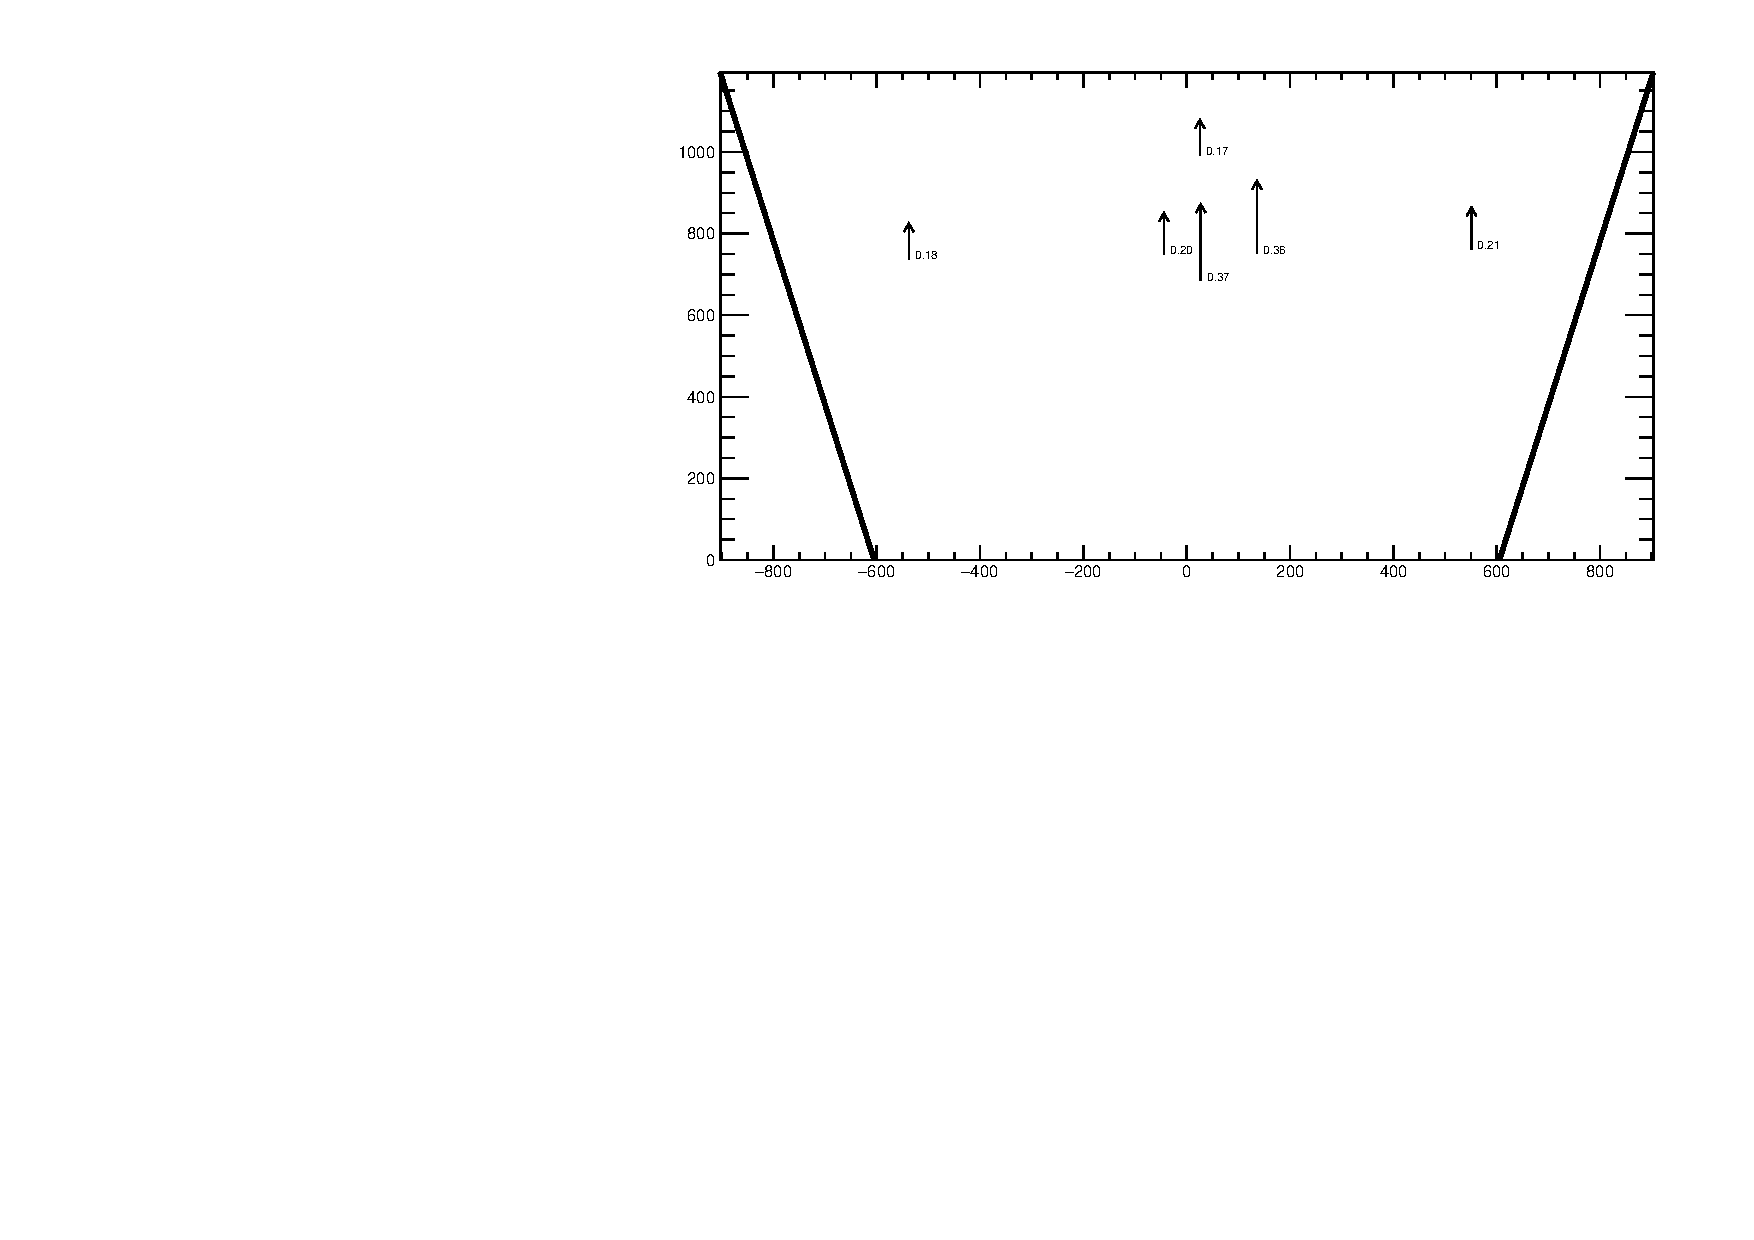
\includegraphics[width=\linewidth]{figures/QL2P11_xray_residuals_layer2_fixedlayers13.pdf}
  \caption{QL2.P.11 x-ray residuals on layer 2, reference layers 1 and 3.}
  \label{fig:xray_res_th2_ql2p11}
\end{subfigure}%
\vspace*{\floatsep}
\begin{subfigure}{\textwidth}
  \centering
  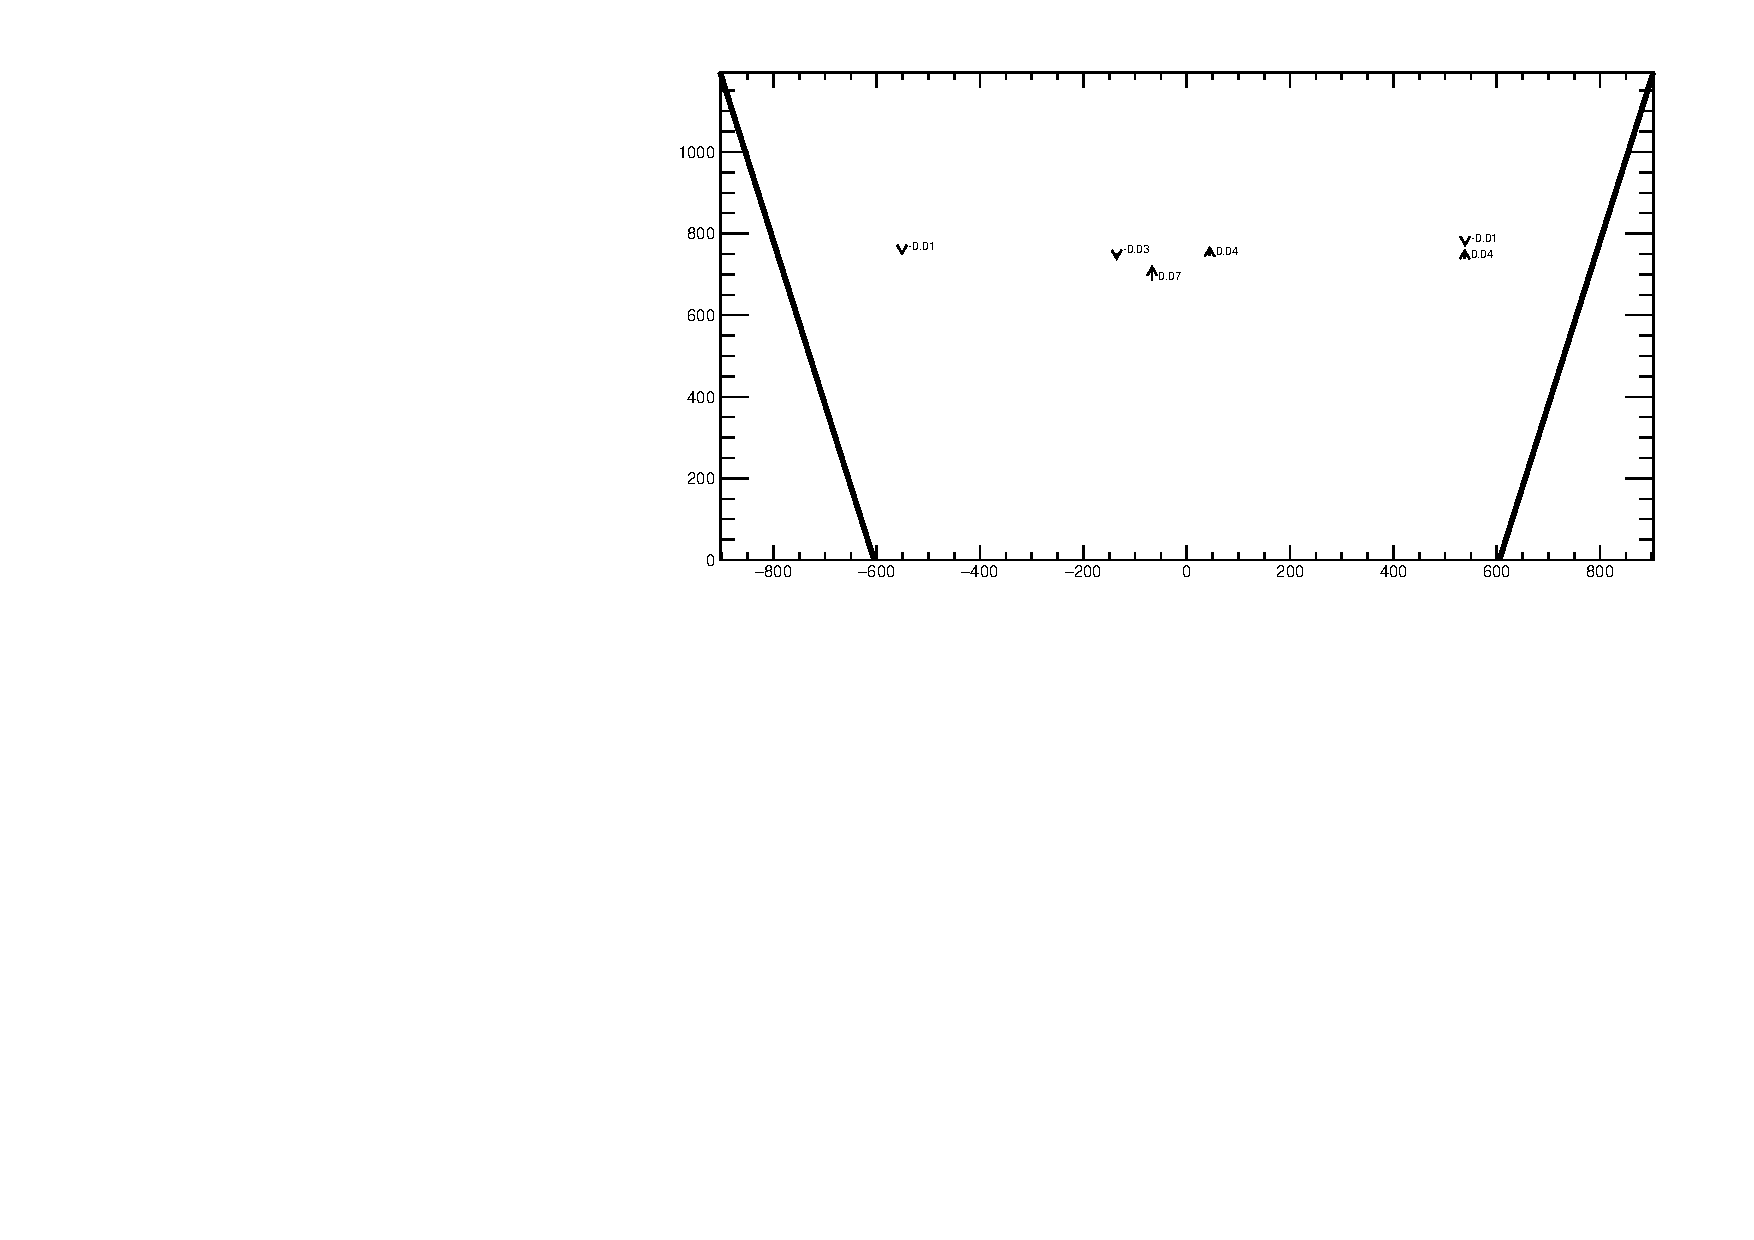
\includegraphics[width=\linewidth]{figures/QL2P08_xray_residuals_layer2_fixedlayers13.pdf}
  \caption{QL2.P.8 x-ray residuals on layer 2, reference layers 1 and 3.}
  \label{fig:xray_res_th2_ql2p8}
\end{subfigure}
\caption{The x-ray residuals on layer 2 calculated from the beam profile centers recorded on layers 1 and 3 for QL2.P.11 and QL2.P.8. The arrows originate from the expected position of the beam profile center assuming a nominal geometry, and the lengths are proportional to the calculated x-ray residuals. The tip of the arrow represents where the recorded hit was with respect to where it should have been recorded nominally. The value of the x-ray residuals are annotated in millimeters and have an uncertainty of $\pm$\SI{0.15}{mm}.}
\label{fig:xray_res_th2}
\end{figure}
\newpage
\restoregeometry

The uncertainty on the x-ray residuals was the error propagated through the tracking, taking an uncertainty of \SI{120}{\micro\meter} on each beam profile center. The uncertainty on the x-ray residuals ranged from \SI{0.15}{mm} to \SI{0.4}{mm} from the most to least geometrically-favourable tracking combination. There is no discernible pattern to the x-ray residuals on QL2.P.8 because they are smaller than the uncertainty. The x-ray residual uncertainties are significantly larger than the uncertainties on the relative local offsets calculated with cosmics data.